\documentclass[sigconf]{acmart}

\usepackage{booktabs} % For formal tables


% Copyright
%\setcopyright{none}
%\setcopyright{acmcopyright}
%\setcopyright{acmlicensed}
%\setcopyright{rightsretained}
%\setcopyright{usgov}
%\setcopyright{usgovmixed}
%\setcopyright{cagov}
%\setcopyright{cagovmixed}


% DOI
%\acmDOI{10.475/123_4}

% ISBN
%\acmISBN{123-4567-24-567/08/06}

%Conference
%MAYBE set this
%\acmConference[WOODSTOCK'97]{ACM Woodstock conference}{July 1997}{El
%  Paso, Texas USA}
%\acmYear{1997}
%\copyrightyear{2016}


%\acmArticle{4}
%\acmPrice{15.00}

% These commands are optional
%\acmBooktitle{Transactions of the ACM Woodstock conference}
%\editor{Jennifer B. Sartor}
%\editor{Theo D'Hondt}
%\editor{Wolfgang De Meuter}


\begin{document}
\title{Linux-Integrated TCP Acceleration as a Service}
%\titlenote{Produces the permission block, and
%  copyright information}
%\subtitle{Extended Abstract}
%\subtitlenote{The full version of the author's guide is available as
%  \texttt{acmart.pdf} document}

\author{Amanda Austin}
\affiliation{
  \institution{University of Texas at Austin}
}
%\email{jsmith@affiliation.org}

\author{Henrique Fingler}
%\authornote{Dr.~Trovato insisted his name be first.}
%\orcid{1234-5678-9012}
\affiliation{
  \institution{University of Texas at Austin}
}
%\email{trovato@corporation.com}


\author{Timothy Stamler}
\affiliation{
  \institution{University of Texas at Austin}
}
%\email{jsmith@affiliation.org}

% The default list of authors is too long for headers.
\renewcommand{\shortauthors}{B. Trovato et al.}


\begin{abstract}
This paper provides a sample of a \LaTeX\ document which conforms,
somewhat loosely, to the formatting guidelines for
ACM SIG Proceedings.\footnote{This is an abstract footnote}
\end{abstract}

%
% The code below should be generated by the tool at
% http://dl.acm.org/ccs.cfm
% Please copy and paste the code instead of the example below.
%
%\begin{CCSXML}
%<ccs2012>
% <concept>
%  <concept_id>10010520.10010553.10010562</concept_id>
%  <concept_desc>Computer systems organization~Embedded systems</concept_desc>
%  <concept_significance>500</concept_significance>
% </concept>
%</ccs2012>
%\end{CCSXML}

%\ccsdesc[500]{Computer systems organization~Embedded systems}
%\ccsdesc[300]{Computer systems organization~Redundancy}
%\ccsdesc{Computer systems organization~Robotics}
%\ccsdesc[100]{Networks~Network reliability}


%\keywords{ACM proceedings, \LaTeX, text tagging}

\maketitle


\section{Introduction}\label{Introduction}

Networking speeds have become faster while CPUs have not, causing network packet
processing efficiency to become important for datacenter networks. Datacenter
applications continue to want high throughput and low latency access to the
network along with the guarantees provided by TCP: lossless in-order delivery of
packets, but this comes at the cost of consuming an increasing fraction of CPU
processing resources. For example, nearly 70\% of packet processing time for a
simple echo server application is spent in the Linux networking stack 
\cite{peter:arrakis}.

To cope with this, many alternative TCP stacks have been proposed that seek to
increase the efficiency of packet processing. TAS (TCP Acceleration as a
Service) splits TCP packet processing into a fast path and a slow path. The fast
path handles common data path operations such as handling in-order delivery of
packets from established connections and generating acknowledgements. The slow
path handles less common, control path operations such as connection management,
congestion control, and connection timeouts. Both the fast path and slow path
operate as user-level processes.

Implementing a TCP stack in userspace comes with a few drawbacks. Namely, the
Linux TCP stack contains a lot of functionality and information about the
network that is hard to replicate in userspace. Ideally, a userspace networking 
stack should make the same decisions about connection management, security,
congestion, etc. as the Linux stack.

We present Linux-Integrated TCP Acceleration as a Service, an extension to TAS
that interfaces with Linux for some slow path operations. The slow path now
sends some packets to Linux, observes Linux's response, and mimics it. In this
way, TAS can gain some of the information and functionality of the Linux TCP
stack, such as firewall and network information (e.g., ARP tables), while
retaining the performance of fast path operations.

Our paper makes the following contributions:

\begin{itemize}
\item We design and implement a method for the TAS to interface with Linux for
  some slow path operations (connection setup and teardown, ARP) in order to
  gain information and functionality.

\item We evaluate our implementation and show that we introduce no overheads
  for fast path operations. Connection setup and ARP slow down significantly,
  but these operations are uncommon enough that they do not affect the
  throughput seen by the application.
\end{itemize}

In the remainder of our paper, we provide some background on TAS and virtual
network devices in Section \ref{Background}. We discuss the design and
implementation of Linux-integrated TAS in Section \ref{Design}. We evaluate
our implementation in Section \ref{Eval} and finally conclude and discuss
future work in Section \ref{Conclusion}.

\section{Background}\label{Background}


* TCP stack types
** kernel
** user level
** hybrid
** other (offload, dedicated cpu)

*split tcp

\begin{figure}
\centering
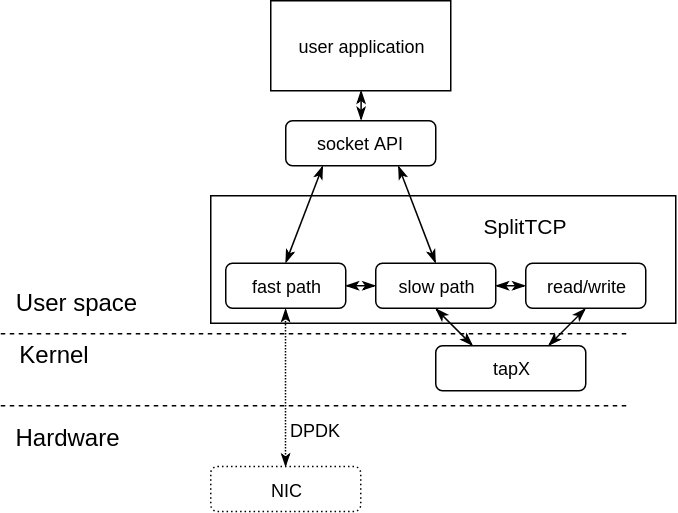
\includegraphics[width=\columnwidth]{figures/splittcp.png}
\caption{TBD.}
\label{fig:splittcp}
\end{figure}


* functionality glue

* Tap devices


\begin{figure}
\centering
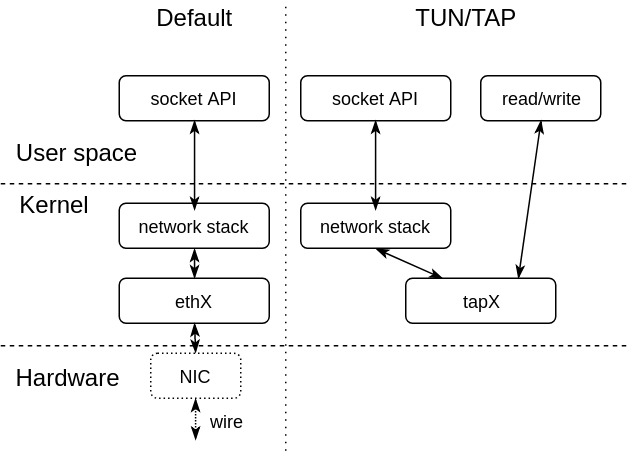
\includegraphics[width=\columnwidth]{figures/tap_diag.png}
\caption{TBD.}
\label{fig:tap}
\end{figure}

\section{Design}\label{Design}

\subsection{TAS Design}

TAS seeks to address a number of problems in the realm of datacenter packet
processing such as efficiency, predictability, and workload proportionality. 
Several important design decisions were made to accomplish these, but we will 
focus on just two of those: the split into a fast path and a slow path, and the
implementation of a userspace TCP stack.

One key way that TAS achieves high connection scalability and 
predictability is by dividing TCP functionality into two components: a fast 
path and a slow path. The fast path handles common-case packets and detects 
exceptions that need to be handled in the slow path. The main functions that
the fast path handles are common case send/receive, where the fast path directly
reads or writes packet payloads from application buffers and interacts directly
with the network, fast ACK handling, where the fast path will either generate or
consume ACK packets quickly without having to invoke the slow path, and 
efficient exception recognition and forwarding. 

In doing this, heavyweight TCP operations are taken out of the data path and 
relegated to the slow path, where they can be handled without affecting the 
performance of other flows in the fast path. The slow path does costly, 
infrequent operations like connection setup and teardown, timeouts, and 
enforcing congestion control. The slow path also handles out of order packets, 
but these are very infrequent in a datacenter environment.
   
In order for this separation and the individual components of the fast path 
and slow path to stay efficient, everything is implemented in a userspace TCP
stack. This provides all the normal functionality of TCP without having to 
switch back and forth between user and kernel space. This is good for 
performance and ease of programming, but isolates the TCP stack from Linux.
While we don't want to rely on Linux for performance operations, it does contain
information about the network and a configurability that would be useful in a 
datacenter environment.

\subsection{Integration Goals}

To most effectively interface with Linux, we take advantage of the previously 
described TAS design choices in order to minimize our impact on common case
packet processing. 

First, we don't make any modifications to the fast path code or data structures.
We prioritize making changes around the fast path, but add no additional lines 
of code to common case packet processing, and no additions and minimal 
interaction with fast path data structures to avoid incurring contention, cache 
problems, or race conditions. By following this rule, we shouldn't incur any
direct overheads to the cases that we care most about.

Secondly, we don't worry about performance in the slow path as long as it
doesn't incur any scheduling or blocking problems with the fast path. We have 
very little control over how often Linux will deliver packets to the slow path, 
so we want to make sure this doesn't negatively affect the fast path threads 
when they might be co-scheduled with the slow path.

\subsection{Compromises Made}

In order to accomplish these goals, we made some compromises to certain problems
in our implementation. In these cases, we could have used few lines of code or 
perhaps gotten better performance for the slow path operation, but at the 
expense of potentially slowing down the fast path.

First, as previously discussed, the fast path naturally consumes all ACK packet,
including during connection setup. In order to most faithfully setup the 
connection, we would need to modify the fast path to either forward ACK packets 
to the slow path, or write packets directly to the tap device. Instead of 
absorbing these costs in the fast path, we instead manually create a new ACK
packet during connection setup in the slow path and write it to the tap device.

Second, we maintain separate sequence numbers between Linux and TAS and 
between TAS and remote hosts. TAS immediately initializes fast path 
state upon receiving a \textit{SYN} packet and doesn't update it after that unless 
there's some kind of exception. Although this takes place in the slow path,
this would require adding some kind of complexity, as we won't know the sequence
number Linux wants to use until it provides a \textit{SYN/ACK}. We can address this by 
doing one of the following: adding an artificial delay or some kind of signal 
from the thread interacting with Linux in the middle of \textit{SYN} processing to make 
sure the sequence number is available when fast path state is initialized, 
initializing fast path state at a later time, modifying the fast path to 
identify either outgoing \textit{SYN/ACK} packets or incorrect outgoing sequence numbers
and adapting, or keeping separate sequence numbers. The final solution ended up 
being the simplest; the first will slow down connection setup even more, the 
second may create additional race conditions or problems in connection setup, 
and the last will slow down the fast path in some way.

Third, similarly to the first compromise, we handle ARP packets manually in 
the slow path, as they are not always forwarded to the slow path. By default,
the fast path only forwards ARP packets to the slow path if it is an IP address
that it doesn't have state for. As connection state is initialized immediately 
upon a \textit{SYN} packet being received, if we try to forward any Linux ARPs to the 
network for that connection, the replies will be dropped by the fast path. In
this case, instead of forwarding all ARP packets to the slow path or delaying
initializing connection state again, we fake ARP responses to Linux requests 
in the slow path by searching TAS's ARP table and manually crafting 
packets. 

\begin{figure}
\centering
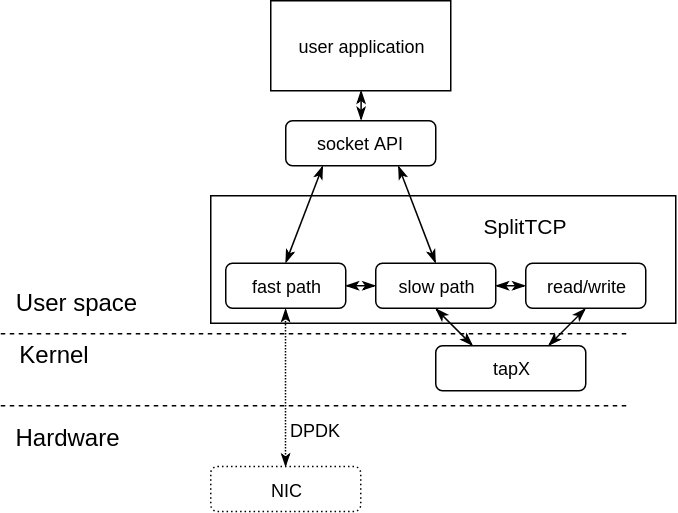
\includegraphics[width=0.7\columnwidth]{figures/splittcp.png}
\caption{Design of TAS with kernel integration. TAS now replicates all slow path operations to the kernel, checks what
it did by reading raw packets from the TAP device and mimics its decisions.}
\label{fig:splittcp_tap}
\end{figure}



\bibliographystyle{ACM-Reference-Format}
\bibliography{paper}

\end{document}
